\begin{normalsize}

\subsection{VDW(3, 2)}
    
Непосредственной проверкой можно убедиться, что $W(3, 2) = 9$.

Но мы докажем худшую оценку(325) --- зато продемонстрируем общую идею доказательства.

Обозначим наши два цвета $R, B$ и рассмотрим произвольную раскраску $\chi: \{1, \ldots, W\} \to \{R, B\}$.

Рассмотрим разбиение $\{1, \ldots, W\}$ на блоки длины $5$ --- можем считать, что $W$ делится на $5$.

$\{1, 2, 3, 4, 5\}, \{6, 7, 8, 9, 10\}, \ldots, \{W-4, W-3, W-2, W-1, W\}$

\subsubsection*{Внутри блока:}

\begin{statement}
    \label{statement:vdw32:1}
    Внутри блока $B_i$: есть арифметическая прогрессия, в которой первые два элемента окрашены одинаково:

    Пусть $B$ --- блок из пяти элементов. Существуют $a, d, d \neq 0$, такие что:

    \[ a, a + d, a + 2d \in B \]

    и

    \[ \chi(a) = \chi(a + d). \]
\end{statement}

\subsubsection*{Раскраска блоков}

Ключевая идея: рассмотреть $32$-раскраску блоков $5$-ми цветов.

\begin{lemma}
    Пусть $W \geq 5 \cdot 33 = 165$. Тогда существует два одинаково раскашенный блока $B_i$ и $B_j,~1 \leq i < j \leq 33$.
\end{lemma}

\begin{theorem}
    Пусть $W \geq 5 \cdot (33 \cdot 2) - 1 = 5 \cdot 65 = 325$. Пусть $\chi: \{1, \ldots, W\} \to \{R, B\}$ --- 2-раскраска $\{1, \ldots, W\}$. Тогда существуют $a, d \in \N$, такие что 

    \[ \chi(a) = \chi(a + d) = \chi(a + 2d) \]
\end{theorem}

\begin{proof}

    Рассмотрим $\{1, \ldots, W\}$ как $65$ блоков длины $5$.

    По лемме существует два одинаково раскрашенных блока $B_i$ и $B_j$, $1 \leq i < j \leq 33$.

    По утверждению $\ref*{statement:vdw32:1}$, внутри $B_i$ существуют $a, d$, такие что $\chi(a) = \chi(a + d)$.

    Пусть $B_i$ и $B_j$ на расстоянии $D$. Так как они одинаково окрашены, то 

    \begin{itemize}
        \item $\chi(a) = \chi(a + d) = \chi(a + D) = \chi(a + D + d) = R$.
        
        \item $\chi(a + 2d) = \chi(a + D + 2d) = B$.
        
        \item $a + 2D + 2d \leq W$.
    \end{itemize}

    \begin{center}
        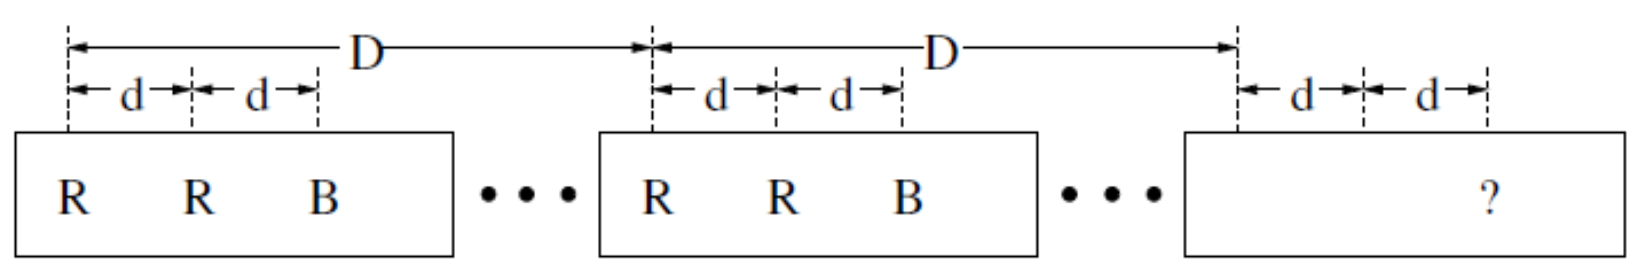
\includegraphics[width=0.7\textwidth]{par48vdw32.png}
    \end{center}

    Если $\chi(a + 2D + 2d) = B$, то 

    \[ \chi(a + 2d) = \chi(a + D + 2d) = \chi(a + 2D + 2d) = B \]

    Если $\chi(a + 2D + 2d) = R$, то

    \[ \chi(a) = \chi(a + D + d) = \chi(a + 2D + 2d) = R \]

    В любом случае получили одноцветную а.п.
\end{proof}


\end{normalsize}